\chapter{Background}
% A more extensive coverage of what's required to understand your work.

% In general you should assume the reader has a good undergraduate
% degree in computer science, but is not necessarily an expert in the
% particular area you've been working on. Hence this chapter may need to
% summarize some ``text book'' material.
%
% This is not something you'd normally require in an academic paper, and
% it may not be appropriate for your particular circumstances. Indeed,
% in some cases it's possible to cover all of the ``background''
% material either in the introduction or at appropriate places in the
% rest of the dissertation.
%
This chapter lays the groundwork for understanding the problem space addressed
by this dissertation. I first explain how scheduling works in Kubernetes,
providing the necessary context for the system architecture. Subsequently, the
chapter delves into \textsc{Pronto}, outlining its core concepts and the
compelling motivations for exploring its application within the Kubernetes
ecosystem. Finally, a review of related Kubernetes schedulers is provided to
highlight the existing landscape and position this work within the current state
of the art.

\section{Kubernetes}

\subsection{Kubernetes Overview}

\begin{figure}[ht]
    \centering
    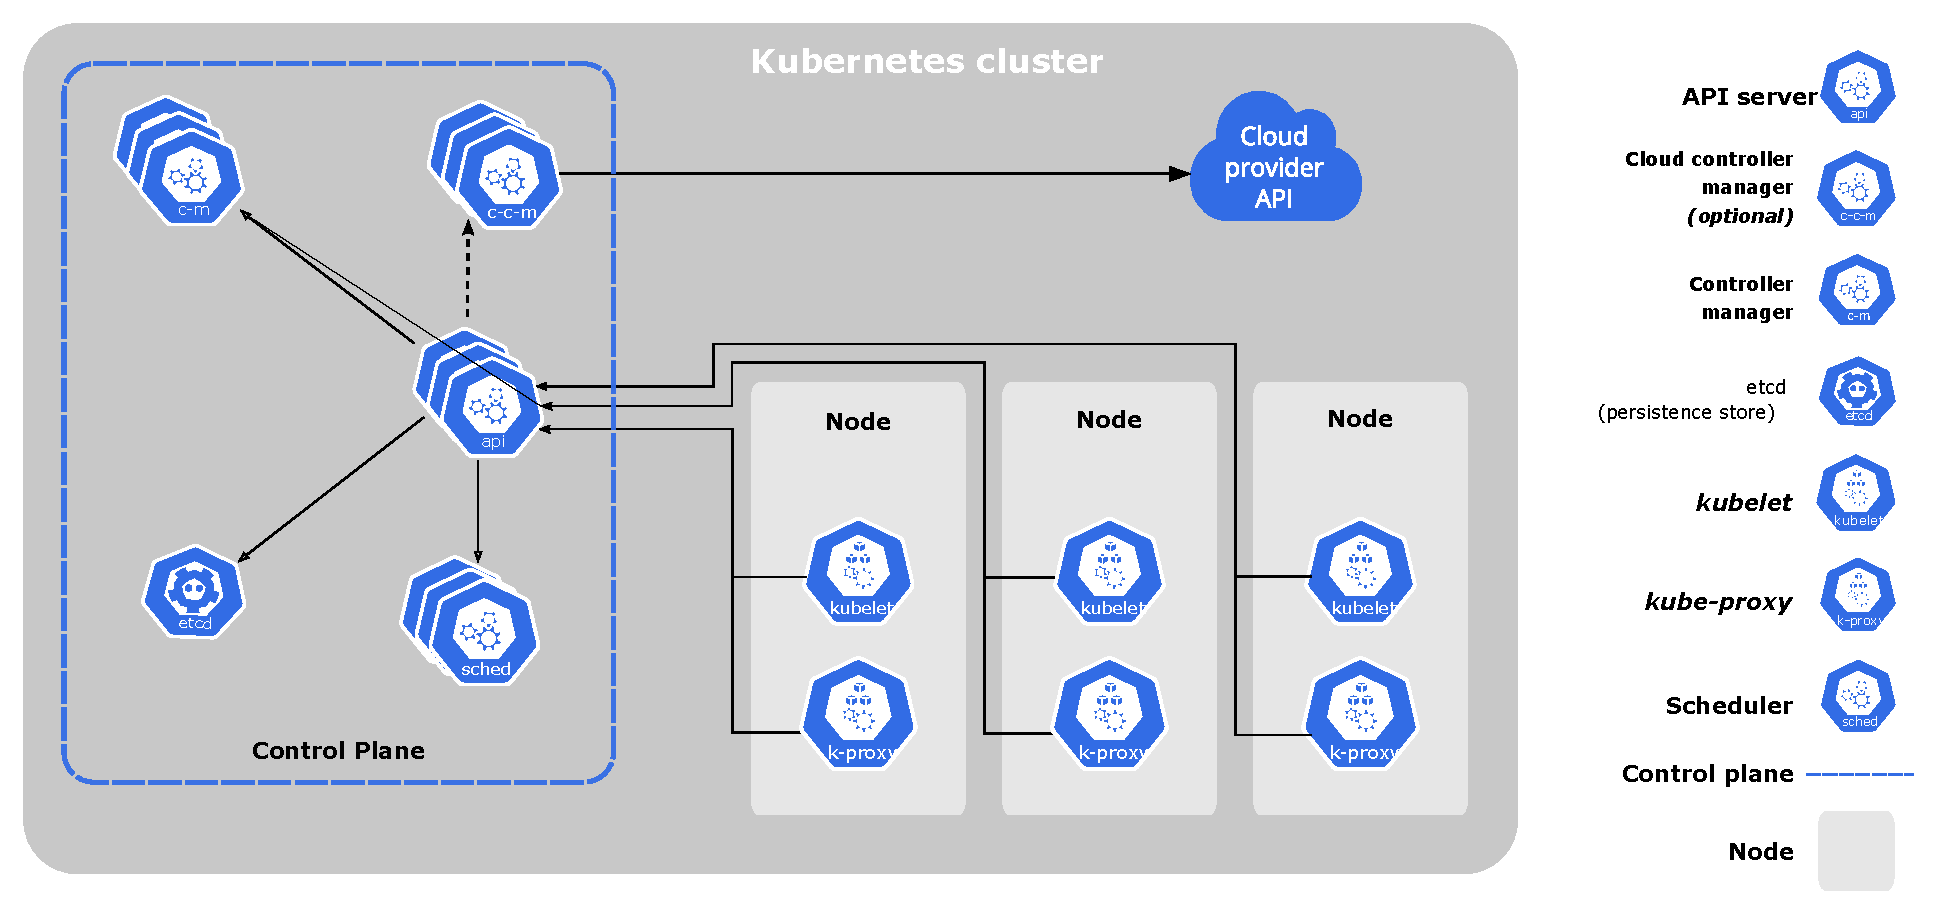
\includegraphics[width=\textwidth]{images/components-of-kubernetes.pdf}
    \caption{The components of a Kubernetes cluster~\cite{kubernetes-components}}
    \label{kube-components}
\end{figure}

A Kubernetes cluster consists of a control plane and one or more worker Nodes.
Components in the control plane manage the overall state of the cluster. The
\verb|kube-apiserver| exposes the Kubernetes HTTP API, which is used to publish
objects such as Deployments, DaemonSets and Jobs. Each
Node in the cluster contains a \verb|kubelet| which manages Pods and ensures
they and their containers are running via a container runtime.

Kubernetes objects are persistent entities in the Kubernetes system. They act as
``records of intent" and describe the cluster's desired state: once created, the
Kubernetes system will constantly work to ensure that the objects exists. The
Kubernetes API is used to create, modify or delete these Kubernetes objects. Almost
every Kubernetes object includes two fields: \verb|spec| and \verb|status|.
\verb|spec| is used on creation as a description of the Objects desired state.
Users can define affinities and QoS classes within this field to influence
scheduling decisions. Containers also contain a \verb|spec| field which
specifies \verb|request| and \verb|limits|. The \texttt{request} field behaves
as a set of minimum requirements and is used when scheduling Pods. In contrast,
the \texttt{limits} field is used by kernel of the Node to throttle a
container's resource usage. \verb|status| describes the current state of the
object, supplied and updated by the Kubernetes system. These fields are core to
scheduling in Kubernetes.

\subsection{Scheduling in Kubernetes}
In Kubernetes, Pods are the smallest deployable units of computing that you can
create and manage. It represents a single instance of a running
process in your cluster and typically contains one or more containers that are
tightly coupled and share resources. Pods can be individually created with their
own Yaml files. However, the Kubernetes API also provides workload objects to
manage multiple pods: these objects represent a higher abstraction level than a
Pod, and the Kubernetes control plane uses the workload's specification to
manage Pod objects on your behalf. Example workloads include Deployment,
StatefulSet, DaemonSet and Job.

When a Pod is created, it initially exists in a ``Pending" state - it has been
declared but hasn't yet been allocated to a Node. Kubernetes schedulers watch for
newly created but unassigned Pods, and based on a set of
rules or algorithms, select the most suitable Node for that Pod. Once a Node is
chosen, the scheduler ``binds" the Pod to the Node, updating the Pod's definition
in the Kubernetes API server by setting its \verb|spec.nodeName| field to the
name of the Node. Once this occures, the Pod transitions from ``Pending" to
``Running".

\section{\protect\textsc{Pronto}}

\subsection{Principle Component Analysis}
This section first explains Singular Value Decomposition (SVD) and how it
relates to solutions of Principal Component Analysis (PCA). I then introduce
Incremental-SVD and Subspace-Merge, which are used to perform FPCA on the stream
of telemetry produced by each Node.

\subsection{Singular Value Decomposition}
The SVD of a real matrix $\mathbf{A}$ with $m$ rows and $n$ columns where $m
\geq n$ is defines as $\mathbf{A} = \mathbf{U}\Sigma\mathbf{V}^T$. Here, $\mathbf{U}$ and
$\mathbf{V}$ are orthogonal matrices of shape $m \times m$ and $n \times n$
containing the left and right singular vecotrs, respectively. $\Sigma$ is a
rectangular matrix of shape $m \times n$ with singular values $\sigma_i$ along
its diagonal~\cite{Strang2009}.
\begin{align}
\mathbf{A} = \begin{bmatrix} a_{11} & \dots & a_{1n} \\ \vdots & \ddots & \vdots
    \\ a_{m1} & \dots & a_{mn} \end{bmatrix} = \begin{bmatrix} \mid & & \mid \\ u_1 & \ldots & u_m
\\ \mid & & \mid  \end{bmatrix} \begin{bmatrix} \sigma_1 & &  & \mid & & \mid \\ &
\ddots & & 0 & \ldots & 0 \\ & & \sigma_m & \mid & & \mid  \end{bmatrix} \begin{bmatrix}
    \text{---} & v_1^T & \text{---} \\ & \vdots & \\ \text{---} & v_m^T & \text{---} \\
    \text{---} & v_{m+1}^T & \text{---} \\ & \vdots  & \\ \text{---} & v_n^T & \text{---}
\end{bmatrix}
\end{align}

SVD can also be written compactly by discarding the elements which do not
contribute to $\mathbf{A}$.
\begin{align}
\mathbf{A} = \begin{bmatrix} \mid & & \mid \\ u_1 & \ldots & u_m
\\ \mid & & \mid  \end{bmatrix} \begin{bmatrix} \sigma_1 &
        & \\ & \ddots & \\ & & \sigma_m \end{bmatrix} \begin{bmatrix} \text{---}
& v_1^T & \text{---} \\ & \vdots & \\ \text{---} & v_m^T & \text{---}
\end{bmatrix}
\end{align}

There always exists the SVD for a real matrix, but the decomposition is not
unique: if $\mathbf{A} = \mathbf{U}_1\Sigma\mathbf{V}_1^T =
\mathbf{U}_2\Sigma\mathbf{V}_2^T$ then $\Sigma_1 = \Sigma_2$ but $\mathbf{U}_1 =
\mathbf{U}_2\mathbf{B}_a$ and $\mathbf{V}_1 = \mathbf{V}_2\mathbf{B}_b$ for some
block diagonal unitary matrices $\mathbf{B}_a,
\mathbf{B}_b$~\cite{eftekhari2019moses, Strang2009}. Each column in
$\mathbf{U}$ and $\mathbf{V}$ is an eignenvector of $\mathbf{AA}^T$ and
$\mathbf{A}^T\mathbf{A}$.

\subsection{Principal Component Analysis}
Pricipal Component Analysis is a staple of linear dimensionality-reduction
techniques. The standard PCA procedure takes as input a matrix $\mathbf{B}$
representing $n$ columns of data with $m$ dimensions. The matrix is first
mean-centered: $\mathbf{A}_{ij} = (\mathbf{B}_{ij} - \mu_i)$ where $\mu_i$ is
the mean of the row $i$. The output of PCA is a set of vectors that explain most
of the variance within $\mathbf{B}$. Given the covariance of the mean-centered
matrix $\mathbf{A}$ is defined as $\mathbf{AA}^T$, the Principal Components (PCs)
maximise the following equation:
\begin{align}
\text{Var}_i = \max_{\substack{x_i \in \mathbb{R}^m \setminus \{\mathbf{0}\} \\
    \|x_i\|=1 \\ x_i \perp x_1 \dots x_{i-1}}} x_i^T \mathbf{A} \mathbf{A}^T x_i
\end{align}

As $\mathbf{A} = \mathbf{U}\Sigma\mathbf{V}^T$ from SVD,
$\mathbf{AA}^T = \mathbf{U}\Sigma\mathbf{V}^T\mathbf{V}\Sigma\mathbf{U}^T =
\mathbf{U}\Sigma^2\mathbf{U}^T$. Therefore, it can be shown that the PCs
$x_i = u_i$ from $\mathbf{U}$. The pair $\mathbf{U}, \Sigma$ will also be
referred to as a subspace as they provide sufficient information to describe the
orginal $\mathbf{B}$ matrix.

\subsection{Subspace-Merge}
Subspace-Merge is used to merge two subspaces together. Given two subspaces
$(\mathbf{U}_1, \Sigma)$ and $(\mathbf{U}_1, \Sigma)$ from $\mathbf{Y}_1$ and
$\mathbf{Y}_2$ respectively, the subspace of $\mathbf{Y} = [\mathbf{Y}_1,
\mathbf{Y}_2]$ is:
\begin{align}
    \mathbf{U}\Sigma = \text{SVD}([\mathbf{U}_1\Sigma_1, \mathbf{U}_2\Sigma_2])
\end{align}
$[\mathbf{A}, \mathbf{B}]$ signifies the concatenation of two matrices with the
same number of rows.

\subsection{Incremental-SVD}
Incremental-SVD allows \textsc{Pronto} to become a streaming algorithm with limited
memory. It takes a stream of chunks $\mathbf{Y}_i$, such that  $[\mathbf{Y}_1,
\ldots, \mathbf{Y}_l] = \mathbf{Y}$, and with each recieved chunk it performs
Subspace-Merge to produce $\mathbf{U}_l, \Sigma_l$ where $\mathbf{Y} =
\mathbf{U}_l\Sigma_l\mathbf{V}_l^T$

\begin{algorithm}
\caption{Incremental-SVD}
\textbf{Data:} $\mathbf{Y} = [\mathbf{Y}_1, \dots, \mathbf{Y}_l]$ \\
    \textbf{Result:} $\mathbf{U}_l, \Sigma_l$ such that $\mathbf{Y} =
    \mathbf{U}\Sigma\mathbf{V}^T$
\begin{algorithmic}
\State $\mathbf{U}_1, \Sigma_1, \mathbf{V}_1^T = \text{SVD}(\mathbf{Y}_1)$
\For {$i = 2$ to $l$}
\State $\mathbf{U}_i, \Sigma_i, \mathbf{V}_i^T = \text{SVD}([\mathbf{U}_{i-1}\Sigma_{i-1}, \mathbf{Y}_i])$
\EndFor
\end{algorithmic}
\end{algorithm}
If the shape of the batches of data is $m \times b$, the space complexity of
Iterative-SVD is $\mathcal{O}(m^2 + mb)$ as only the latest version of
$\mathbf{U}_i,\Sigma_i$ and $\mathbf{Y}_i$ are needed for each iteration.

\subsection{FPCA and FSVD}
FPCA combines the relationship between standard SVD and PCA with the
Subspace-Merge operation, to calculate the PCs of the data $[\mathbf{Y}_1,
\ldots,\mathbf{Y}_m]$ from $m$ nodes. Every node $i$ performs perform SVD  on
their local data, to produce the subspace $\mathbf{U}_i, \Sigma_i$. These
subspaces can be merged using at most $m-1$ Subspace-Merges to obtain the global
subspace $\mathbf{U}'\Sigma'$, corresponding to the PCs of the aggregated data
from all the nodes. \textsc{Pronto} turns this procedure into a streaming algorithm, by
running Subspace-Merge on the subspaces produced by incremental-SVD. Finally,
\textsc{Pronto} also introduces a forgetting factor $\gamma$ in front of
$\mathbf{U}_i\Sigma_i$ in Incremental-SVD that allows it to ``forget" old data
by gradually reducing the influence of previous subspaces. Like with standard
PCA, FPCA can be considered as FSVD on mean-centered data.

\subsection{Low-Rank Approximations}
It can be shown that using the first $r$ eignenvectors in the above algorithms
approximate the result of using all $m$ eignenvectors, i.e. if
\begin{align}
\mathbf{Y} = \begin{bmatrix} \mid & & \mid \\ u_1 & \ldots & u_m
    \\ \mid & & \mid  \end{bmatrix} \begin{bmatrix} \sigma_1 &
        & \\ & \ddots & \\ & & \sigma_m \end{bmatrix} \begin{bmatrix} \text{---}
& v_1^T & \text{---} \\ & \vdots & \\ \text{---} & v_m^T & \text{---}
\end{bmatrix}
\end{align}
We can use $\mathbf{U}^r = \begin{bmatrix} \mid & & \mid \\ u_1 & \ldots & u_r
    \\ \mid & & \mid  \end{bmatrix}$ and $\mathbf{\Sigma}^r = \begin{bmatrix}
\sigma_1 & & \\ & \ddots & \\ & & \sigma_r \end{bmatrix}$ where $r \leq m$ in
Incremental-SVD and Subspace-Merge. This lets \textsc{Pronto} reduce the number of
computations it performs and its memory usage.

\subsection{\protect\textsc{Pronto} System Overview}
\begin{figure}[ht]
    \centering
    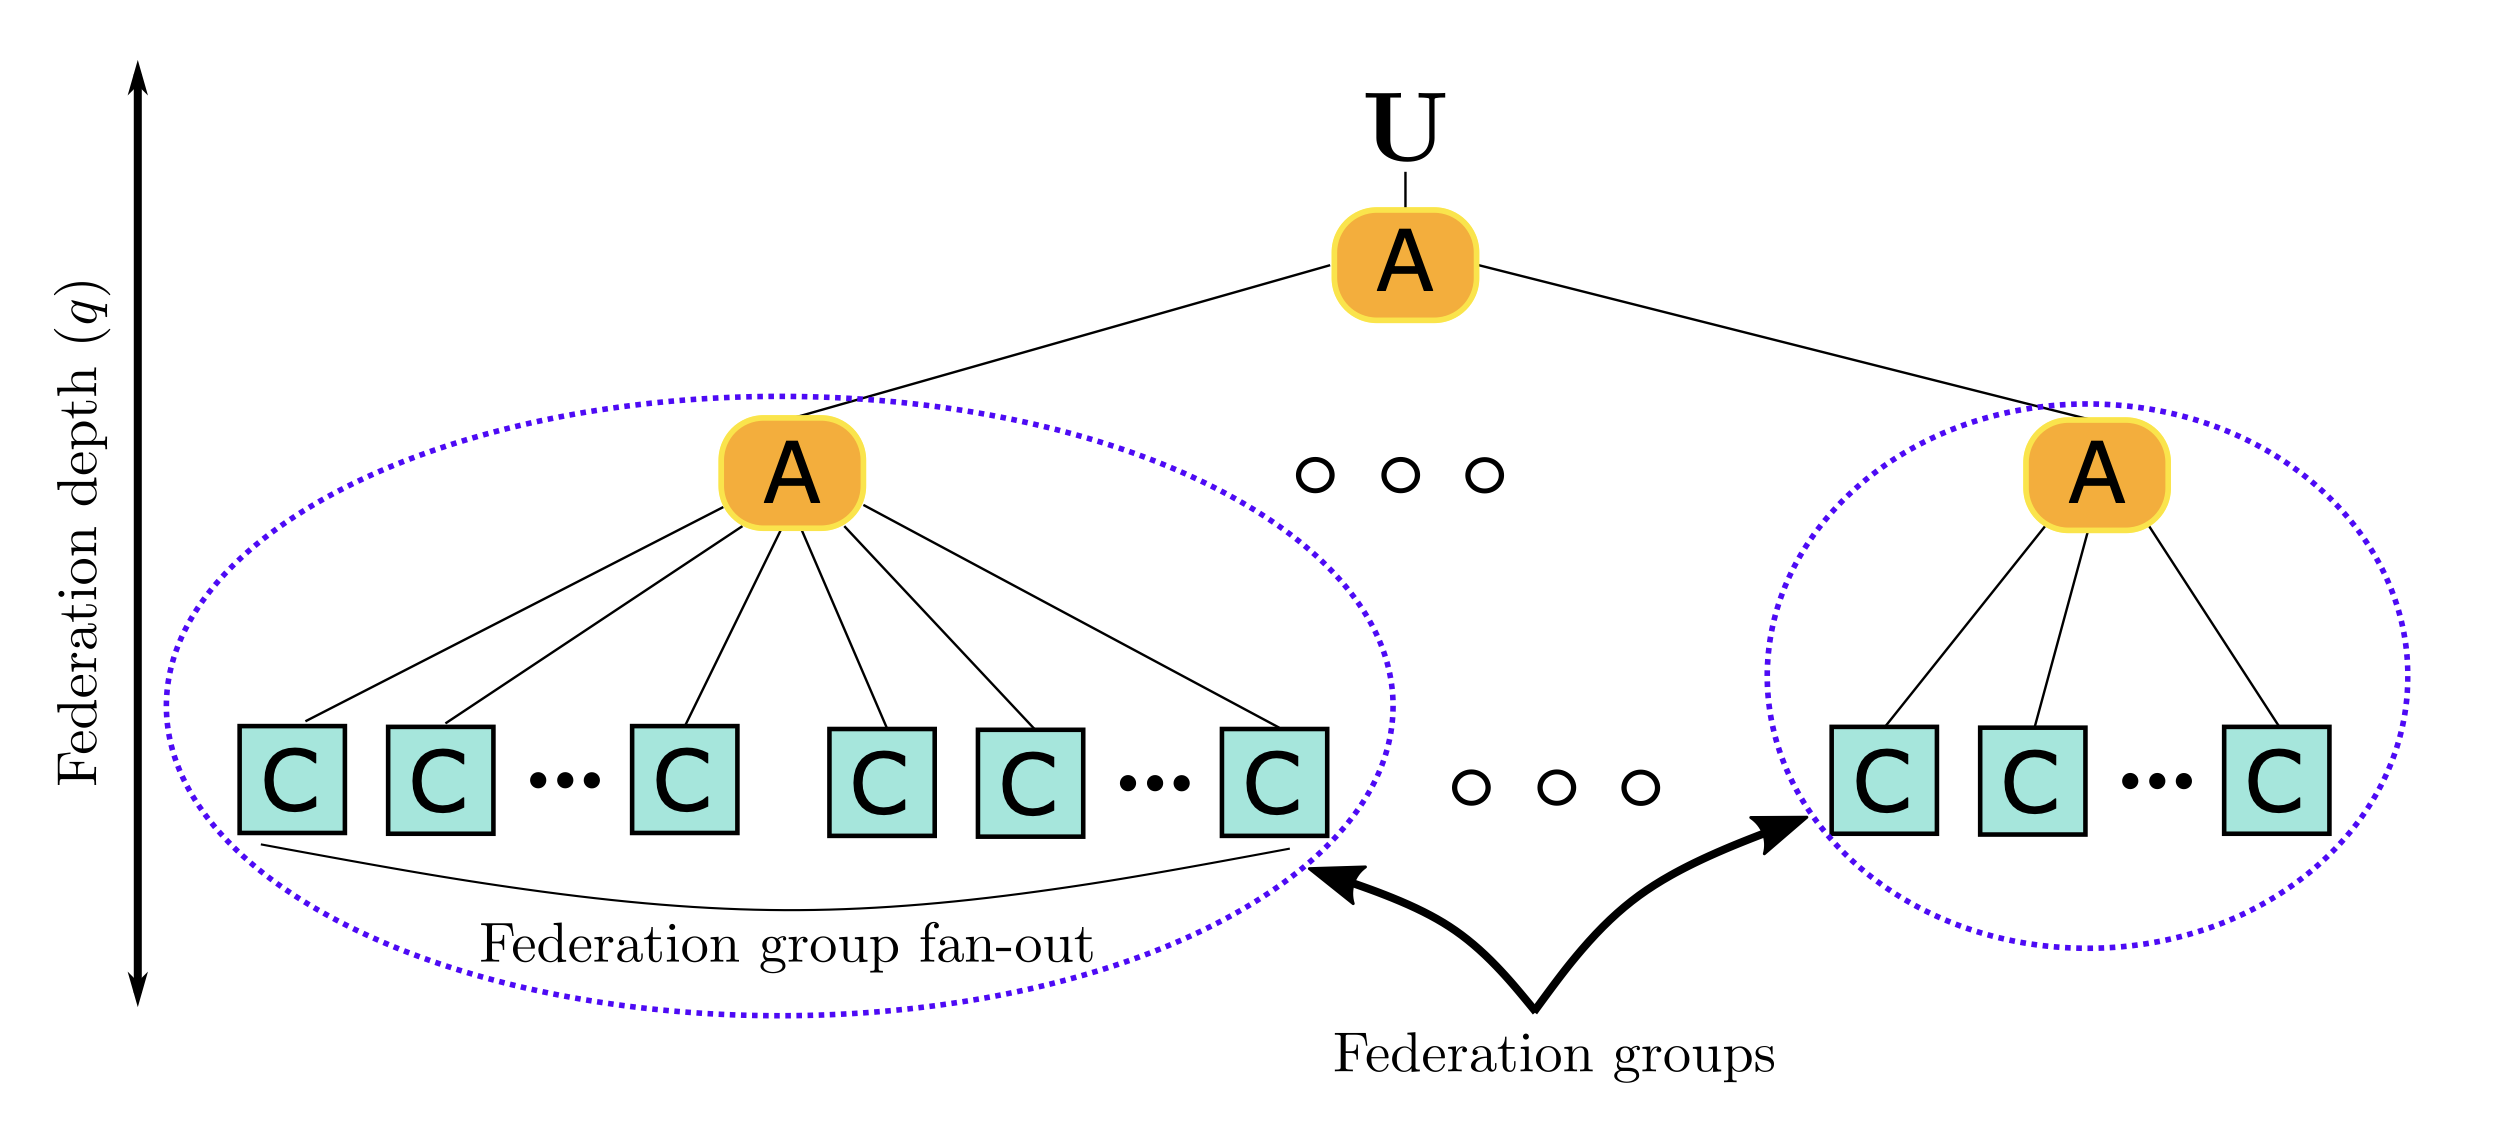
\includegraphics[width=\textwidth]{images/pronto-agg.png}
    \caption{How local models are aggregated in \textsc{Pronto}. Dedicated aggregator
    nodes propagate the updated subspaces until the root is reached~\cite{grammenos_pronto_2021}.}
    \label{pronto-agg}
\end{figure}
There are two types of nodes in \textsc{Pronto}: compute node (C) and aggregator node
(A). Compute nodes collect and center node statistics (i.e. CPU and Memory) and
perform Incremental-SVD to obtain the low rank approximations of the local
subspace $\mathbf{U},\Sigma$. The aggregator nodes before Subspace-Merge on
incoming subspaces, with subspace produced by the root aggregator node being
propagated back to the compute nodes.

\subsection{\protect\textsc{Pronto} Reject-Job Signal}
\begin{figure}[ht]
    \centering
    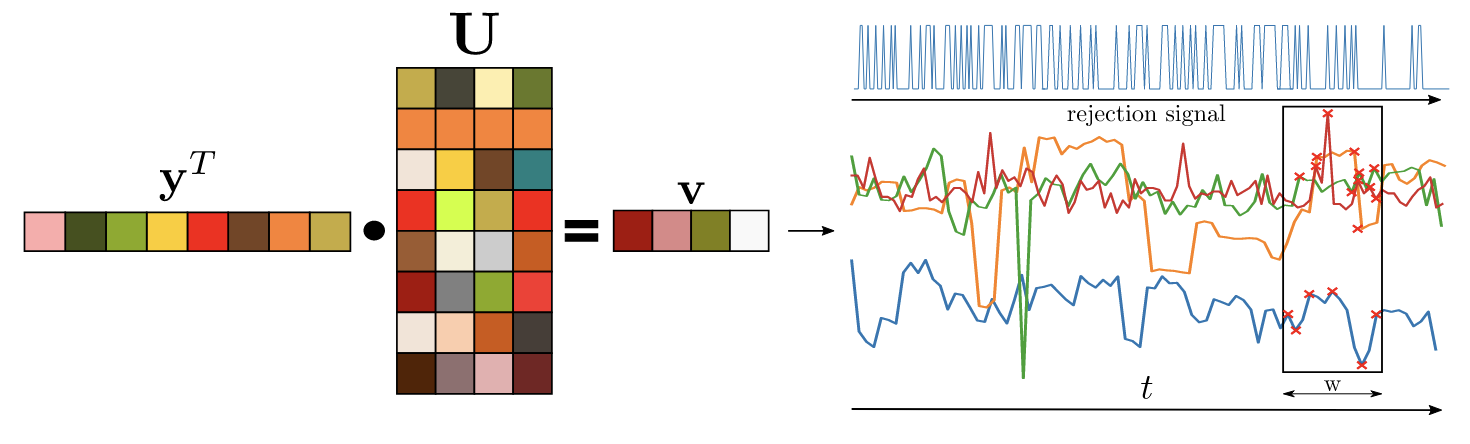
\includegraphics[width=\textwidth]{images/pronto}
    \caption{Projection of incoming $y \in \mathbb{R}^d$ onto embedding $U \in
    \mathbb{R}^{d \times r}$ producing $R$ projections in $v \in \mathbb{R}^{1
    \times r}$. Projections are tracked over time for detecting spikes which
    form the basis of the rejection signal. The sliding window for spike
    detection for each projection is of size $w$ also shown in the figure.}
    \label{pronto-components}
\end{figure}

Each compute node projects their data onto the latest version of $\textbf{U}$,
and identifies all the spikes. If the weighed sum of these spikes, using the
corresponding singular values in $\Sigma$, exceeds a threshold, a rejection
signal is raised to indicate that the node is potentially experiencing
performance degradation and a job should not be scheduled on that node.

\subsection{Strengths}
\textsc{Pronto}'s core strength is its ability to leverage global telemetry data
to predict performance degradation with high accuracy. The orginal
\textsc{Pronto} paper~\cite{grammenos_pronto_2021}, which compared its
effectiveness against non-distributed dimensionality-reduction methods,
demonstrated superior performance in predicting CPU-Ready spikes in real-world
datacenter traces. This improved accuracy over the non-distributed
strategies suggests that significant correlations exist between the resource
usages of different jobs across various nodes at the same point in time. This
federated approach allows for a more comprehensive understanding of system-wide
resource contention, providing more accurate contention predictions than with
only individual node data. These compelling results indicate a strong potential
benefit from applying \textsc{Pronto} underlying principles to a Kubernetes
environment where efficient resource management is paramount.

\subsection{Weaknesses}
\label{sec:intro-weakness}
While \textsc{Pronto} offers a promising approach to perforamnce prediction, its
direct application within Kubernetes scheduling environment faces significant
challenges due to fundamental assumptions and practical limitations of its
original design.

\subsubsection{Assumptions}
The \textsc{Pronto} paper primarily focuses on a method for measuring node
"responsiveness" to future workloads, yielding a binary Reject-Job signal.
However, implementing its design in a complex system like Kubernetes raises
fundamental challenges:
\begin{enumerate}
    \item \textbf{Zero-Latency Assumption:} A critical assumption in the
        \textsc{Pronto} paper is the absence of communication latency, and
        implicitly binding latency within the system. This implies that
        scheduled workloads are immediately reflected in the telemetry, and thus
        the signal. In such a scenario, a central scheduler could
        instantaneously stop assigning workloads once a Node signal potential
        degredation. However, this assumption does not hold in real-world
        Kubernetes clusters. The latency between a pod being bound to a Node and
        that Pod actually starting to run and consume resources has been shown
        to reach as high as 4 seconds \cite{qadeer_scaling_2022}. Directly
        applying \textsc{Pronto}'s binary signal in this high-latency
        environment could lead to a ``runaway train" schenario": Nodes might
        advertise willingness to accept new Pods while a large number of
        ``inflight" Pods are still pending startup and will overload the node
        once active.
    \item \textbf{Lack of Explicit Alloction Algorithm:} \textsc{Pronto} allows
        indivdual compute nodes to reject or accept incoming jobs. However, it
        does not explicitly provide a system to optimally decide which compute
        nodes are considered for a task. While a simple approach would be to allow
        individual Nodes to request Pending Pods, it suffers from scalability
        issues as hundreds of Nodes sending requests to the Kubernetes APIServer
        would greatly degrade its performance or even cause it to crash.
        Instead, I decided to take a centralised approach, where Nodes
        periodically update their signal to influence where Pods are allocated.
    \item \textbf{Limited Scoring Capability:} Unlike typical Kubernetes
        schedulers that emply a scoring-function to rank Nodes and select the
        ``optimal" fit~\cite{kube-scheduler}, a binary signal offers no
        mechanism to differentiate between suitable Nodes. This could lead to
        suboptimal allocation decisions, potentially reducing overall cluster
        throughput and efficiency
\end{enumerate}
These issues raise the need for a more sophisticated signal that is:
\begin{enumerate}
    \item \textbf{Comparable:} provides enough information to score and rank
        Nodes effectively.
    \item \textbf{Reservable:} allows the scheduler to track the pending impact
        of previous scheduling decisions until Pods have begin running.
\end{enumerate}

% The Pronto paper implements a binary "responsiveness" signal which predicts
% upcoming performance degradation. Because the authors assume a system with no
% communication latency (implicitly assuming that scheduled workloads were
% immediately visisble in the signal as well), they could send this signal
% directly to a central scheduler which could then stop assigning workloads once a
% node sent a Reject Signal.
%
% However, due to significant pod startup latency, the method can't be used in a
% real-world Kubernetes cluster is infeasible. When measuring pod startup in a
% 100 node clusters, the more than 50\% of pods took more than $\approx$ 1 second
% to startup. In addition, when nodes were 100\% full, pod startup could reach up
% to 4 seconds. This latency is significant when Kubernetes schedulers can
% support a throughput of $\approx$1000 pods per second
% \cite{qadeer_scaling_2022}. Applying the same approach as used in the paper,
% could result in nodes advertising a "willingness" to take on new pods while
% a large number of pods are in "flight" and once running will immediately
% overload the node. To prevent this runaway train type problem, I need to define
% a reservation function: a function that reserves an amount of the signal for a
% bound pod. This is necessary to allow previous scheduling decisions to have an
% imnpact on the signal while the signal updates to take into account the
% scheduled pods.
%
% In addition, telemetry-based schedulers can use individual node performance
% information to score and fine-tune pod allocations. A binary signal does not
% provide the necessary information for scoring nodes, potentially resulting in
% worse pod allocations.
%
% In summary, the requirements of the signal are:
% \begin{itemize}
    % \item Reservable: the scheduler must be able to track the pending impact of
        % previous scheduling decisions until the pods have begun running.
    % \item Comparable: the signal must provide enough information to score nodes
% \end{itemize}

\subsubsection{Peak-Prediction}
\textsc{Pronto} relies on peak-detection within contention metrics (originally
CPU-Ready in VMware vSphere) to predict future performance degradation. For
\textsc{Pronto} to generate an accurate Reject-Job signal in Kubernetes, the
chosen contention metrics should exhibit clear, distinguishable spikes during
genuine high-resource contention. While increasing the number of collected
metrics can help reduce the impact of erroneous spikes, collecting more
telemetry and operating on larger matrices will incurr additional overheads and
reduce the number of tasks a Node can accept before valid contention is
detected.

Linux-based systems offer Pressure Stall Information (PSI) metrics, accessible
via \texttt{/proc/pressure/<cpu|memory|io>}. These pseudo-files track the time
tasks are stalled waiting for resources. To investigate the feasibility of using
PSI for peak prediction within a Kubernetes Node, I polled the polled the
\verb|/proc/pressure| files under different workloads.

\begin{figure}[ht]
    \centering
    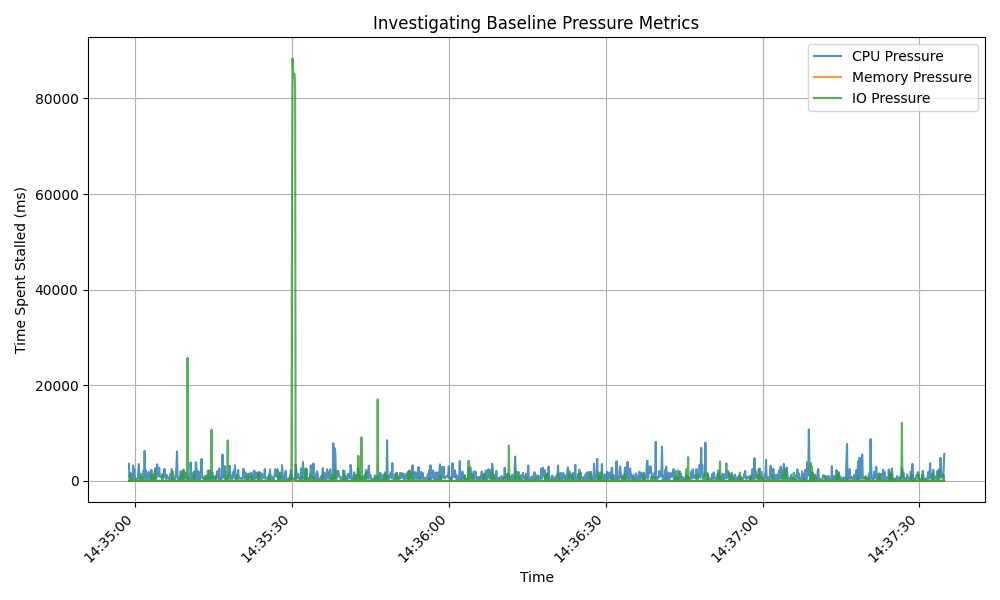
\includegraphics[width=0.48\textwidth]{images/pressure-baseline.png}
    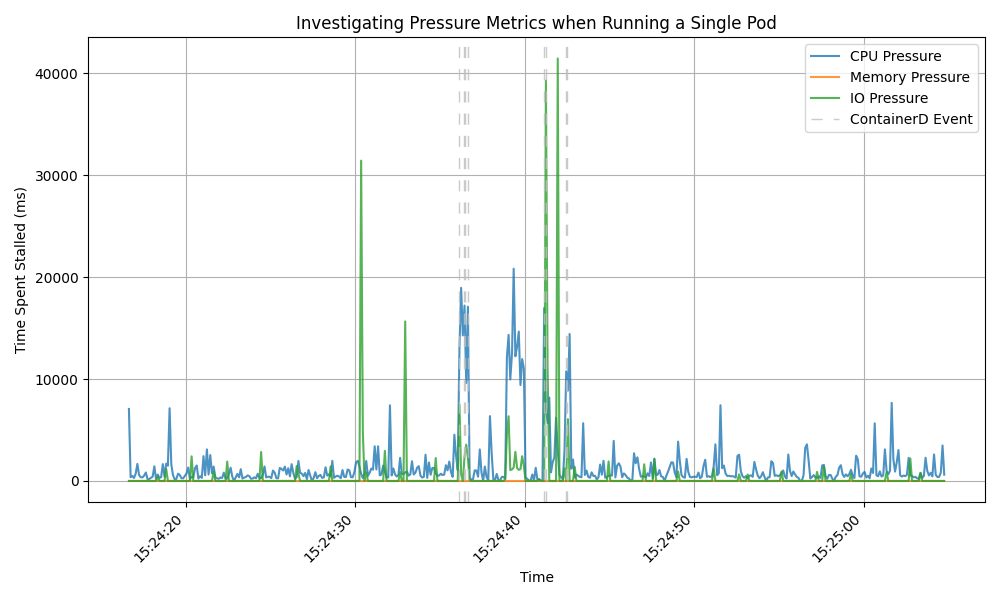
\includegraphics[width=0.48\textwidth]{images/pressure-single.png} \\
    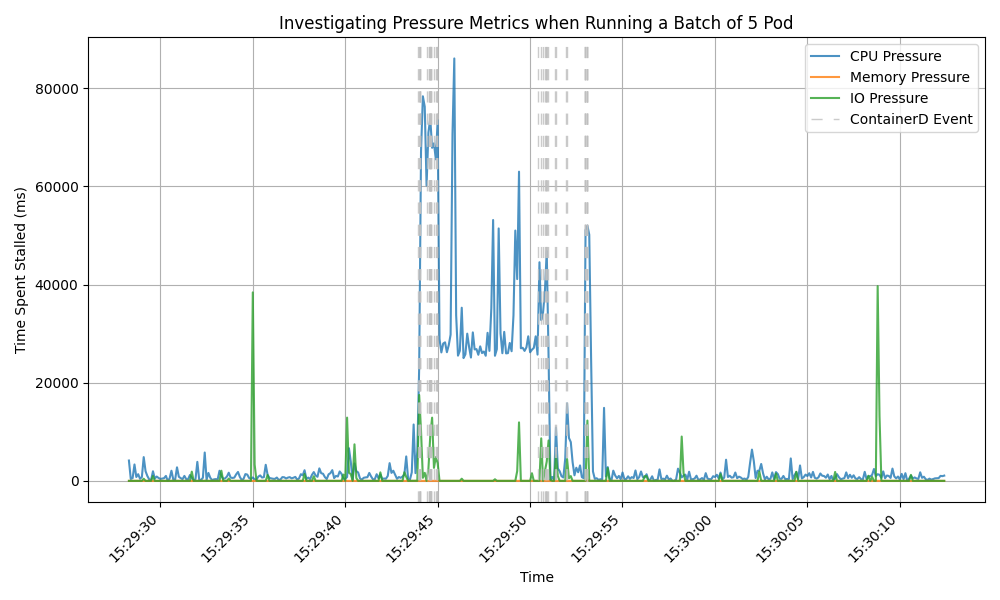
\includegraphics[width=0.48\textwidth]{images/pressure-smallbatch.png}
    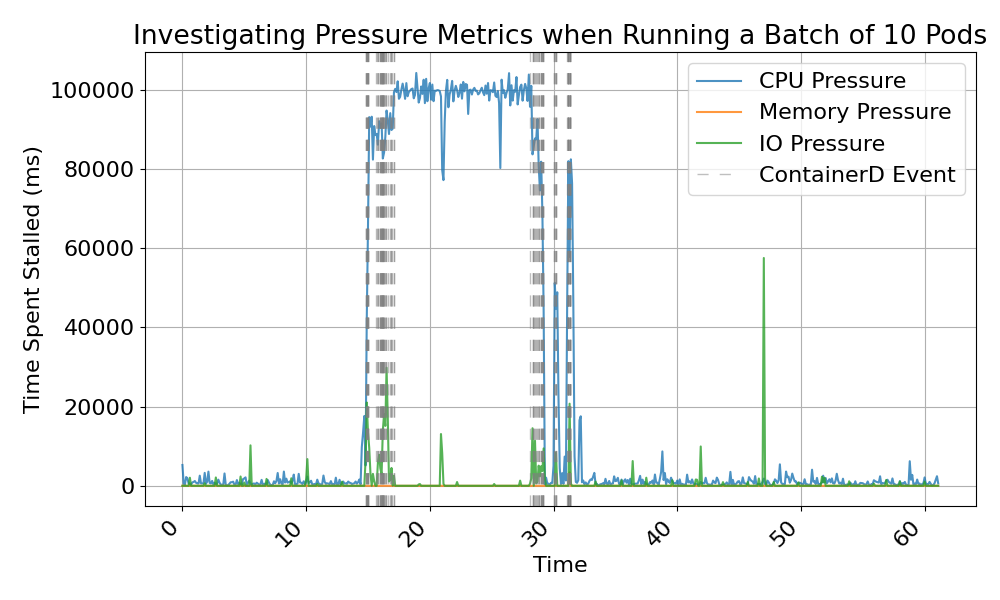
\includegraphics[width=0.48\textwidth]{images/pressure-bigbatch.png}
    \caption{Measurements of \texttt{total} from \texttt{/proc/pressure/} under
    different loads. The container runtime results in spikes no matter the
    workload.}
    \label{fig:pressure}
\end{figure}

As demonstrated in Figure \ref{fig:pressure}, even with lightweight workloads,
the PSI metrics frequently experience significant spikes. These transient spikes
can be attributed to the container runtime (e.g. Containerd) consuming resources
during the creation or deleteion of containers. These ``noise" would be
difficult to distinguish from genuine indicators of resource conention ,
compromising the accuracy of \textsc{Pronto}'s peak-detection mechnanism.

\begin{figure}[ht]
    \centering
    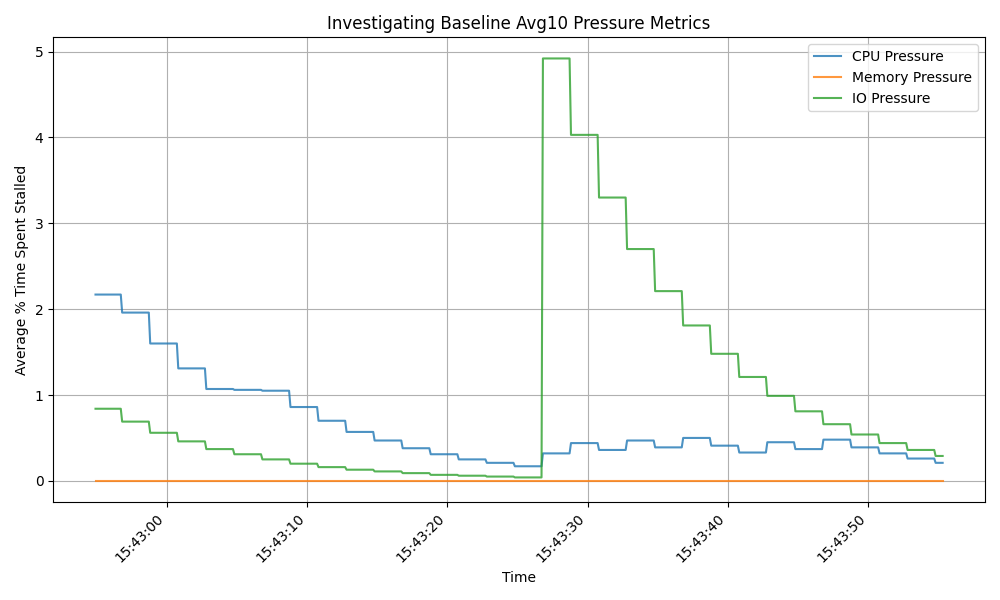
\includegraphics[width=0.48\textwidth]{images/avg-pressure-baseline.png}
    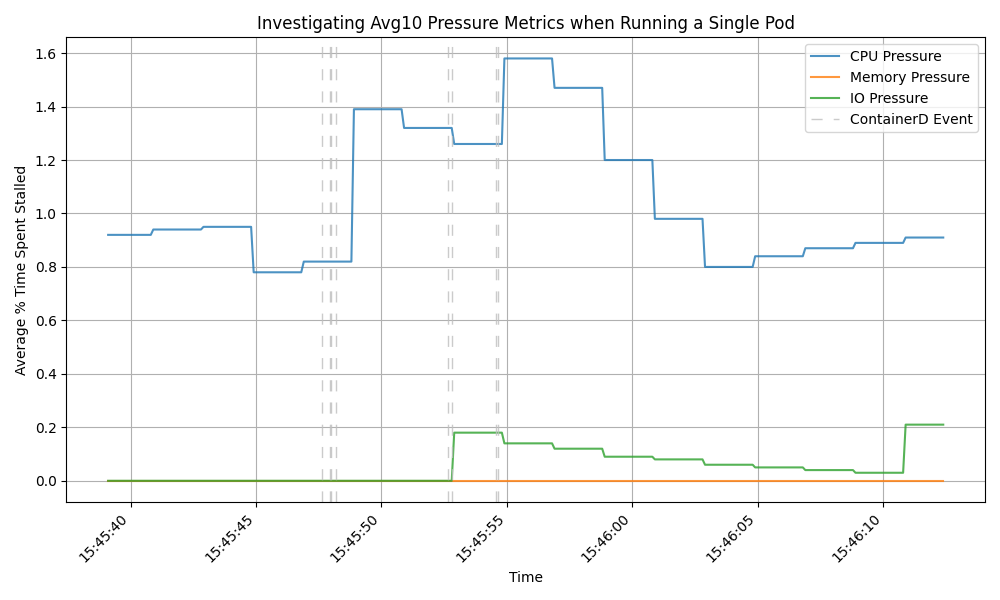
\includegraphics[width=0.48\textwidth]{images/avg-pressure-single.png} \\
    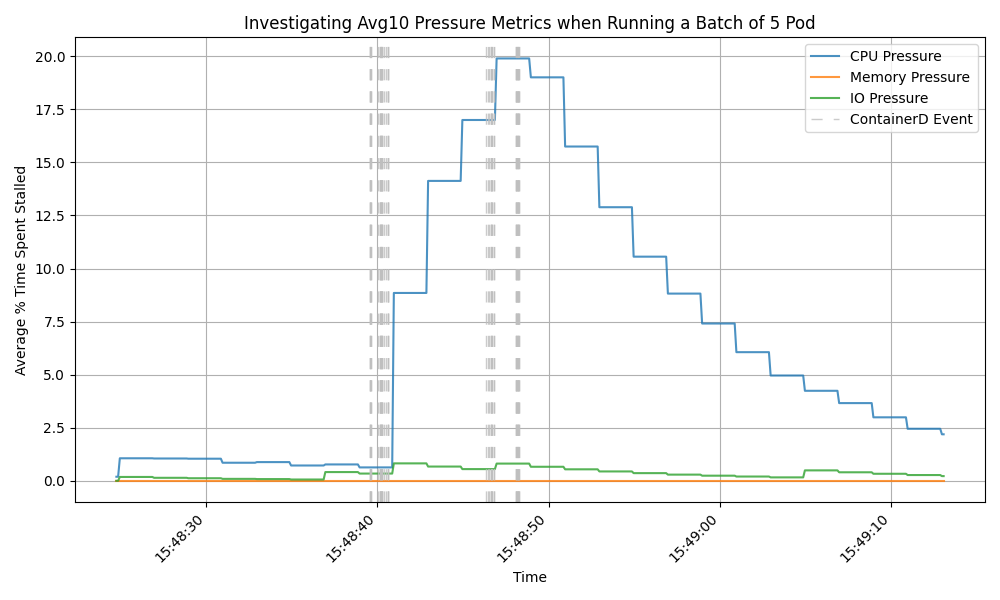
\includegraphics[width=0.48\textwidth]{images/avg-pressure-smallbatch.png}
    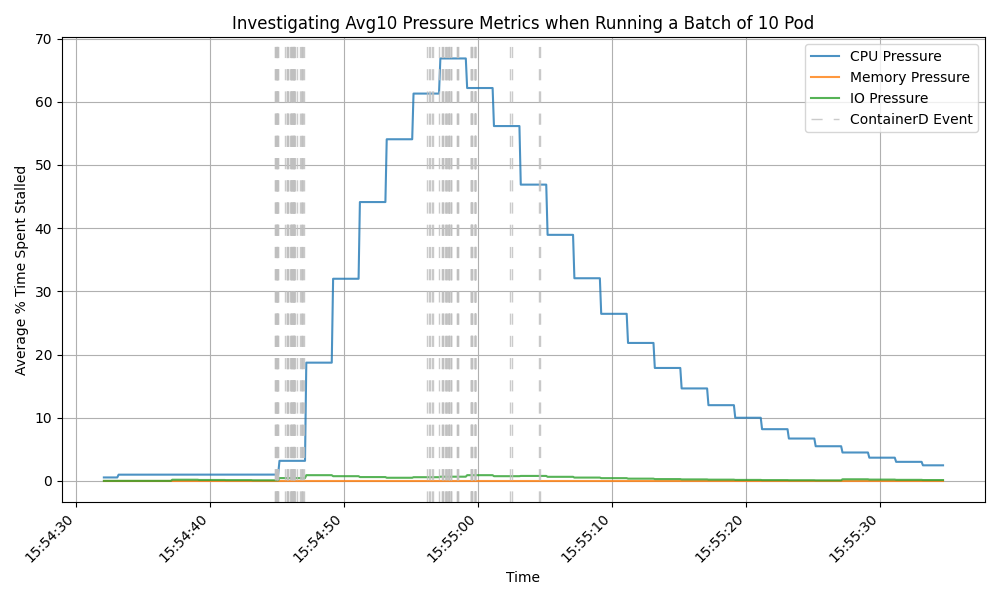
\includegraphics[width=0.48\textwidth]{images/avg-pressure-bigbatch.png}
    \caption{Measurements of \texttt{avg10} from \texttt{/proc/pressure/} under
    different loads. The container runtime results in spikes no matter the
    workload.} \label{fig:pressure-avg}
\end{figure}
The PSI metrics also expose an average over a 10-second window. Figure
\ref{fig:pressure-avg} illustrates that averaging the PSI metrics can indeed
reduce the impact of these container runtime-induced spikes. However, this
smoothing comes at the cost of responsiveness. In the experiments with a 10-pod
batch, the averaged metrics failed to converge on the true value observed in
Figure \ref{fig:pressure} before the Pods had finished running. 10 seconds in
the timeframe of Kubernetes can result in the same ``runaway train" situation
described earlier.

Based on this early empirical investigation, I conclude that direct
preak-prediction from sub-second polling of raw PSI metrics, can not be easily
applied within a fast-paced Kubernetes environment.


% In the paper, Pronto uses \verb|CPU-Reeady| which is generated by the VMware
% vSphere virtualisation platform. This metric can't be used within a
% Kubernetes cluster as machines can be both virtual and physical. Since Linux
% 4.20+, the kernel can track how long tasks are stalled waiting for the CPU
% at a cgroup granularity. By inspecting the the root cgroup’s CPU pressure
% file using \verb|cat /proc/pressure/cpu| you can measure the total time all
% processes spent waiting for the CPU to be available.
%
% While this type of metric can be used to alert of performance degradation,
% this metric has a few shortcomings. Firstly, it only reports CPU-centric
% information. This is not always representative measure of resource
% contention as memory-heavy workloads may starve for RAM resources while
% metrics like \verb|CPU-Ready| and \verb|/proc/pressure/cpu| remain
% unaffected.
%
% Secondly, a significant amount of resources are used starting up or deleting
% containers. This results in large spikes, as shown in figure
% \ref{pressure-eval}, which are difficult to distinguish from genuine CPU-Ready
% spikes. As Pronto uses spike detection to predict future resource performance
% degradation, container start-ups could produce detectable spikes which would
% reduce the rate at which pods are assigned to nodes and could result in lower
% throughput.
%


\section{Related Work}
This section examines existing Kubernetes schedulers, highlighting
those that share characteristics with \textsc{Pronto}: distributed and federated
schedulers, online schedulers, performance-aware schedulers, and machine
learning-based schedulers.

\subsection{Federated and Distributed Scheduling}
\textsc{Pronto} is described as a federated algorithm that executes plans in a
decentralised fashion. Each computing node makes independent decisions for task
assignments without needed global synchronisation. This contrasts with
monolithic centralised schedulers~\cite{kube-scheduler, gog_firmament_2016},
such as the default Kubernetes scheduler (\texttt{kube-scheduler}), which acts
as a single dispatcher on the master node and has a global state view. These
schedulers can suffer from scalabilitity issues, reliance on cached data and
increased network traffic~\cite{grammenos_pronto_2021}. Research has been done
in multi-cluster scheduling and cluster federation, addressing challenges in
scalability and geo-distributed environments. Examples include frameworks like
KubeFed~\cite{faticanti2021application} and architectural proposals like
Foggy~\cite{santoro2017foggy}. Although \textsc{Pronto} immediate focus s on
scheudling within a network of nodes that might not be geographically dispersed
or owned by different entities, its federated learning approach to scharing
knowledge through aggregated iterates is relevant to discussions around
decentralised control and coordination in distributed infrastructures.

\subsection{Online, Real-Time, and Streaming Scheduling}
TODO: THIS SECTION FEELS WEAK, I MAY DELETE
\textsc{Pronto} is designed for online task scheduling and operates on real-time
performance. As a streaming algorithm, \textsc{Pronto} processes incoming data
in a single pass without storing historical information, enabling Nodes to make
immediate scheduling decisions about incoming workloads. While the default
Kubernetes scheduler reacts to changes, it performs bin-packing with statically
defined resource requests and capacity. Research outside of Kubernetes has
repeatedly shown that analysing large-scale performance data in near real-time
for efficient scheduling is difficult~\cite{grammenos_pronto_2021}. As a result,
\textsc{Pronto}'s explicit streaming algorithm enabling low-latency scheduling
decisions distinguishes it from approaches that might involve more substantial
processing pipelines, offline techniques or the reliance on potentially stale
cached information.

\subsection{Performance-Aware and Predictive Scheduling}
As a performance-aware scheduler, \textsc{Pronto} employs
dimensionality-reduction technique to efficiently process the vast amount of
telemetry data produced by each node, with the goal of predicting performance
degradation. While, CPU and RAM utilisation are common metrics for
performance-aware Kubernetes schedulers~\cite{bao2019deep, beltre2019kubesphere,
bestari2020dynamic, carvalho2021qoe, toka2021ultra}, \textsc{Pronto}
distinguishes itself as the first scheduler to incorporate CPU-Ready for task
scheduling.

Furthermore, the dynamic nature of Kubernetes workloads strongly suggest that
predictive techniques could improve scheduling efficiency and resource
utilisation~\cite{carrion2022kubernetes}. Traditional forecasting methods (such as
exponential smoothing, ARIMA, and SVM) were also explored in
\cite{grammenos_pronto_2021} for CPU Ready spike prediction, but were found to
have worse accuracy. This still remains an open research topic.

\subsection{Machine Learning-Based Schedulers}
\textsc{Pronto} exploits unsupervised learning technique, specifically Federated
PCA, to discover hidden correlations within unstructured high-dimensional
telemetry data. Machine Learning (ML) algorithms  are increasingly adopted in
scheduling to learn from data and improving decision quality.
Reinforcement learning-based schedulers \cite{bao2019deep, huang2020rlsk,
peng2021dl2, han2021tailored} use reward functions to continuously improve
scheduling decisions. While, ML has been used before to predict application or
resource utilisation~\cite{yang2019design, carvalho2021qoe,
harichane2020proposal}, these schedulers are typically domain-specific.
\textsc{Pronto}'s application of unsupervised PCA to predict the performance
of a Node represents a novel use-case of ML with broad applications within the
scheduling domain.

\subsection{Summary of Related Work}
In summary, \textsc{Pronto} distinguishes itself within the Kubernetes
scheduling landscape through its federated and decentralised approach, enabling
independent decision-making at the node level. Its streaming algorithm allows
for immediate, low-latency task assignments. As a performance-aware scheduler, it
innovatively uses CPU-Ready for task scheduling and applies unsupervised
Federated PCA for predictive insights, offering a distinct machine learning
approach.

\section{Summary}
This chapter provided the foundational knowledge for the dissertation,
introducing an overview of the Kubernetes architecture and its scheduling
mechnaism. It then introduced \textsc{Pronto}, a novel approach to scheduling,
explaining the core mathematics behind its FPCA, and highlighting its accuracy
in predicting performance degredation through global telemetry. However,
significant weaknesses were identified, emphasising the necessity for a more
sophisticated \textbf{comparable} and \textbf{reservable} signal. Finally, a
review of existing Kubernetes schedulers, helped distinguish \textbf{Pronto}
from the current landscape and highlight it potential contribution.

% \begin{tcolorbox}[boxsep=0mm,left=2.5mm,right=2.5mm]
    % \textbf{Summary:} {\em In this chapter I will summarise the problem and
    % problem space. I will review the findings of the related work, highlighting
    % weaknesses of existing Kubernetes schedulesr with respect to QoS
    % scheduling.}
% \end{tcolorbox}

